\section{Simulation Outcomes}\label{Sec: Simulation Outcomes}

This section presents the simulation outcomes for two specific cases: the flow of charged particles around a sphere and the behavior of ions in a grid potential layout similar to those found in gridded electrostatic ion thrusters. These simulations are evaluated by examining energy conservation within the system, serving as a key indicator to verify the plausibility of the results. Furthermore, the steady state of the simulation is introduced, where key properties of the system, such as mass, momentum, energy, and charge, become time-invariant. This condition defines the point at which further iterations no longer provide significant changes to the results, indicating the simulation has reached equilibrium. Lastly, the limitations of the current implementation of the electrostatic particle-in-cell (\acs{ES PIC}) method are outlined and demonstrated through a specific challenge encountered during simulation.

\subsection{Flow Around a Sphere}\label{Sec: Flow Around Sphere}

In this section, a sphere with a fixed potential of $\Phi = -100V$ is introduced within the simulation domain, as illustrated in Fig. \ref{fig: Sphere simulation domain}. Oxygen ions (O+) with a single positive charge are injected from the inlet on the left plane, maintaining a particle density of \SI{1e10}{\per\meter^3} and a drift velocity of 7000 m/s. The sphere serves as a particle sink, absorbing ions upon interaction. As a result, a condensed stream forms behind the sphere, characterized by a region of increased ion density. This phenomenon arises due to the lensing effect, where the sphere deflects ion trajectories, concentrating them in the region downstream \cite{brieda_plasma_2019}.

\begin{figure}[H]
    \centering
    \begin{subfigure}[b]{0.49\linewidth}
        \centering
        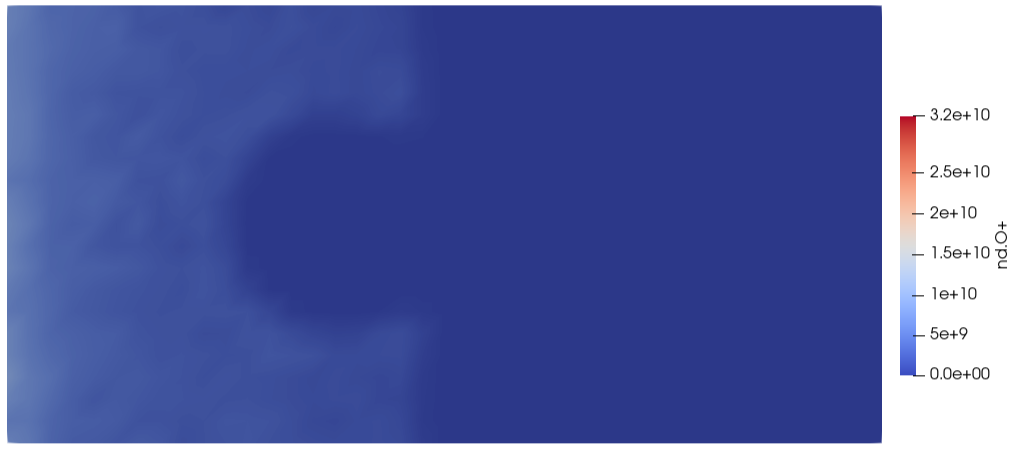
\includegraphics[width=\linewidth]{figures/Sphere/80_iterations.png}
        \caption{80 Iterations}
        \label{fig:average_iteration_time}
    \end{subfigure}
    \hfill
    \begin{subfigure}[b]{0.49\linewidth}
        \centering
        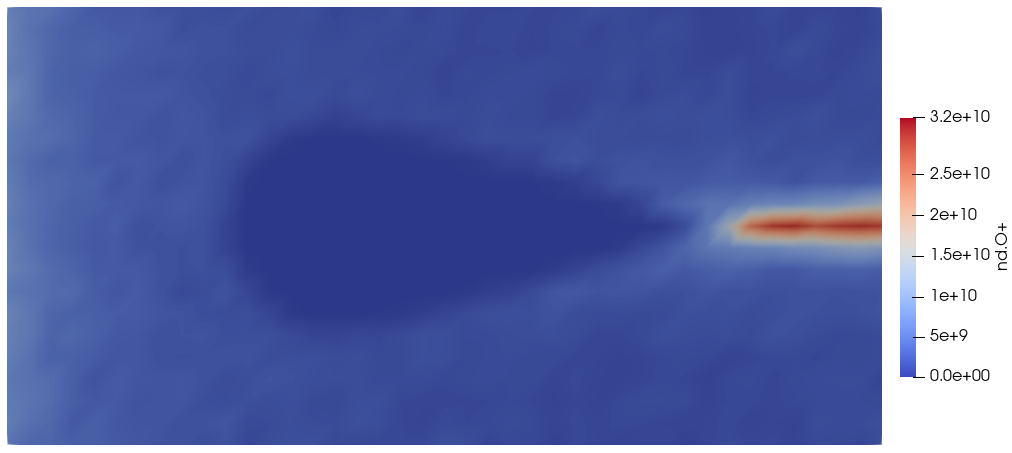
\includegraphics[width=\linewidth]{figures/Sphere/160_iterations.png}
        \caption{160 Iterations}
        \label{fig:average_iteration_count}
    \end{subfigure}
    \caption{Comparison of Average Iteration Time and Count with Relaxation Values}
    \label{fig:comparison}
\end{figure}


steady state 

only changes through noise introduced by the randomized injection of particles!

Therefore some fluctuations


\begin{figure}[H]
    \centering
    \begin{subfigure}[b]{0.49\linewidth}
        \centering
        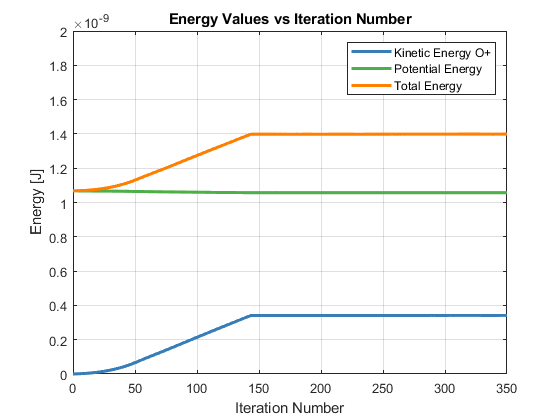
\includegraphics[width=\linewidth]{figures/Sphere/energy_values_plot.png}
        \caption{Energy}
        \label{fig:average_iteration_time}
    \end{subfigure}
    \hfill
    \begin{subfigure}[b]{0.49\linewidth}
        \centering
        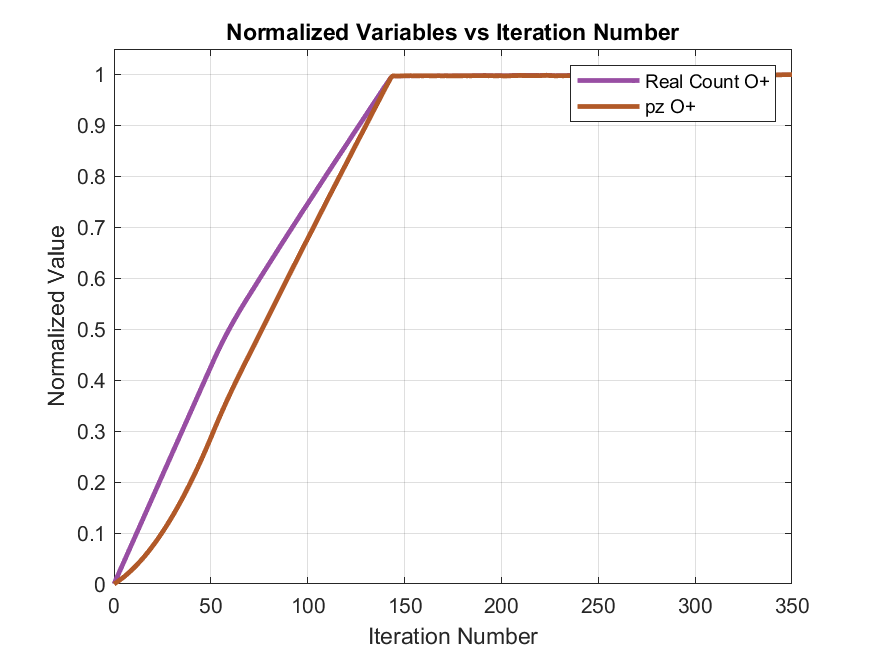
\includegraphics[width=\linewidth]{figures/Sphere/normalized_variables_plot.png}
        \caption{other variables}
        \label{fig:average_iteration_count}
    \end{subfigure}
    \caption{Comparison of Average Iteration Time and Count with Relaxation Values}
    \label{fig:comparison}
\end{figure}

Expected results the potential energy resulting from the grids remains constant in the system

however the kinetic energy and therefore the the total energy in the system increases until the steady state is achieved.

This happens after roughly 145 iterations at which point the total amount of particles in the system remains the same.

Those outcomes are consistent with the results presented for a similar simulation outlined in \cite{brieda_plasma_2019}.

\subsection{Basic Framework for Grid Potential Layout in RIT Thruster Design}



\begin{figure}[H]
    \centering
    \begin{subfigure}[b]{0.49\linewidth}
        \centering
        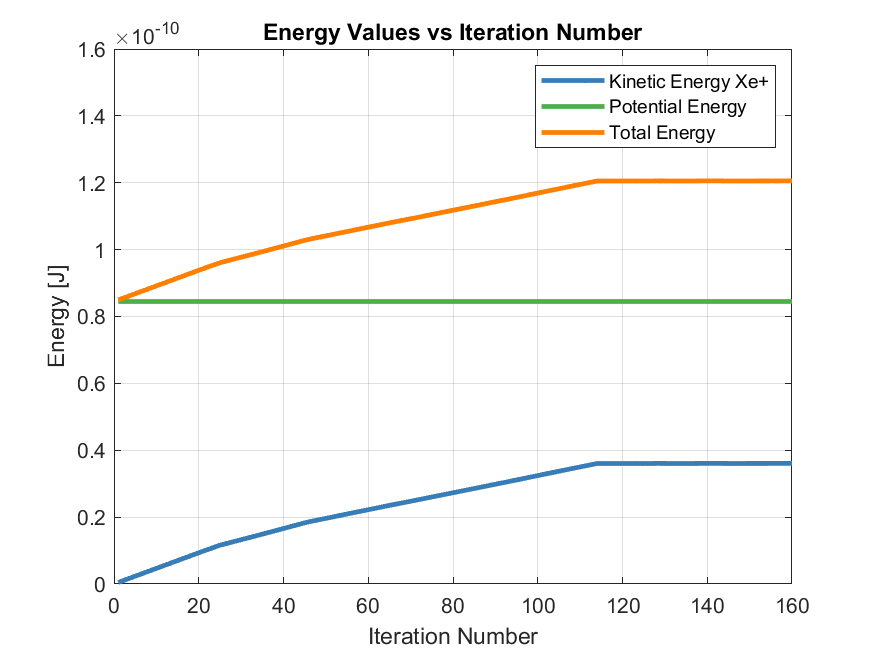
\includegraphics[width=\linewidth]{figures/GIT/energy_values.png}
        \caption{Energy}
        \label{fig:average_iteration_time}
    \end{subfigure}
    \hfill
    \begin{subfigure}[b]{0.49\linewidth}
        \centering
        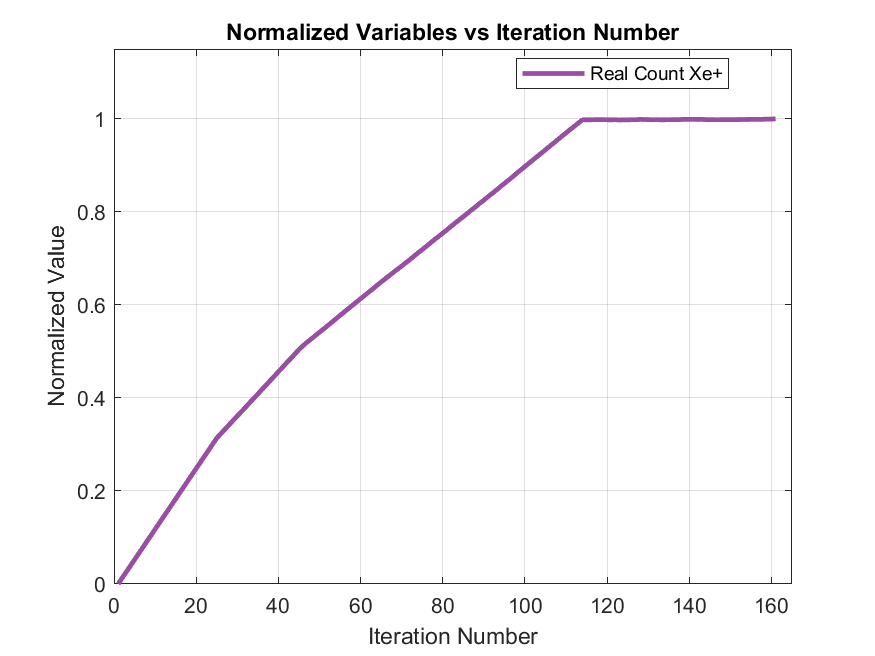
\includegraphics[width=\linewidth]{figures/GIT/normalized_variables.png}
        \caption{other variables}
        \label{fig:average_iteration_count}
    \end{subfigure}
    \caption{Comparison of Average Iteration Time and Count with Relaxation Values}
    \label{fig:comparison}
\end{figure}


